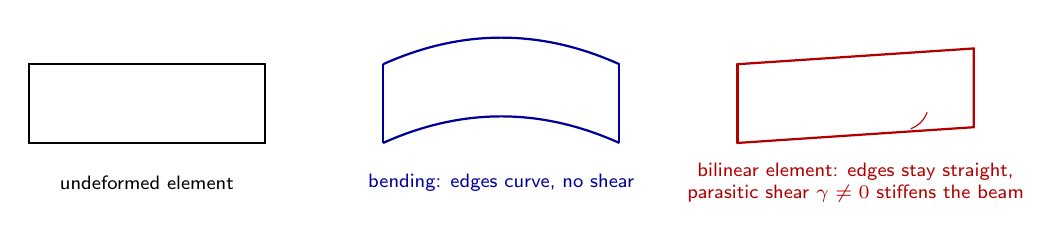
\begin{tikzpicture}[font=\sffamily\scriptsize]
\draw[thick] (0,0) -- (3,0) -- (3,1) -- (0,1) -- cycle;
\node at (1.5,-0.5) {undeformed element};
\draw[thick,blue!60!black] (4.5,0) .. controls (5.5,0.45) and (6.5,0.45) .. (7.5,0);
\draw[thick,blue!60!black] (4.5,1) .. controls (5.5,1.45) and (6.5,1.45) .. (7.5,1);
\draw[thick,blue!60!black] (4.5,0) -- (4.5,1); \draw[thick,blue!60!black] (7.5,0) -- (7.5,1);
\node[blue!60!black] at (6.0,-0.5) {bending: edges curve, no shear};
\draw[thick,red!70!black] (9,0) -- (12,0.2) -- (12,1.2) -- (9,1) -- cycle;
\draw[thick,red!70!black] (9,0) -- (9,1);
\draw[red!70!black] (11.2,0.18) arc (-70:-20:0.35) ;
\node[red!70!black,align=center] at (10.5,-0.5) {bilinear element: edges stay straight,\\parasitic shear $\gamma\ne0$ stiffens the beam};
\end{tikzpicture}
